% ======================= CHAPTER IV =======================
\chapter{Results}\label{ch:results}

\section{Hardware Developement}

The hardware for the TTE communication system, named MAGIC \textit{MAG-netic Induction Communication}, was designed and built to meet a specific set of requirements and constraints. First, the system must be able to pass the proof of concept test by achieving communication over a medium but significant distance in an underground environment. Additionally, the equipment must not be excessively bulky or heavy to facilitate its transport and versatility.
\newp
The communication system is defined primarly by the magnetic coupling principe between two resonant coils, one used as transmitter and the other as receiver. Also the system has to be bidirectional, so both coils can work as transmitter or receiver depending on the comunication direction.
\subsection{Design}

The TTE communication system comprises several elements that work together to transmit and receive data via magnetic induction. The main element is the resonant coil, which is designed to generate and receive magnetic fields at a specific frequency. In addition to the coil, the system includes an amplifier to boost the transmitted message and a switching system to change the resonant coil's connection between the system's input and output channels, depending on the desired communication direction (TX or RX).
\newp
Here is a conceptual diagram of the complete system in figure \ref{fig:system-diagram}.

\begin{figure}[H]
    \centering
    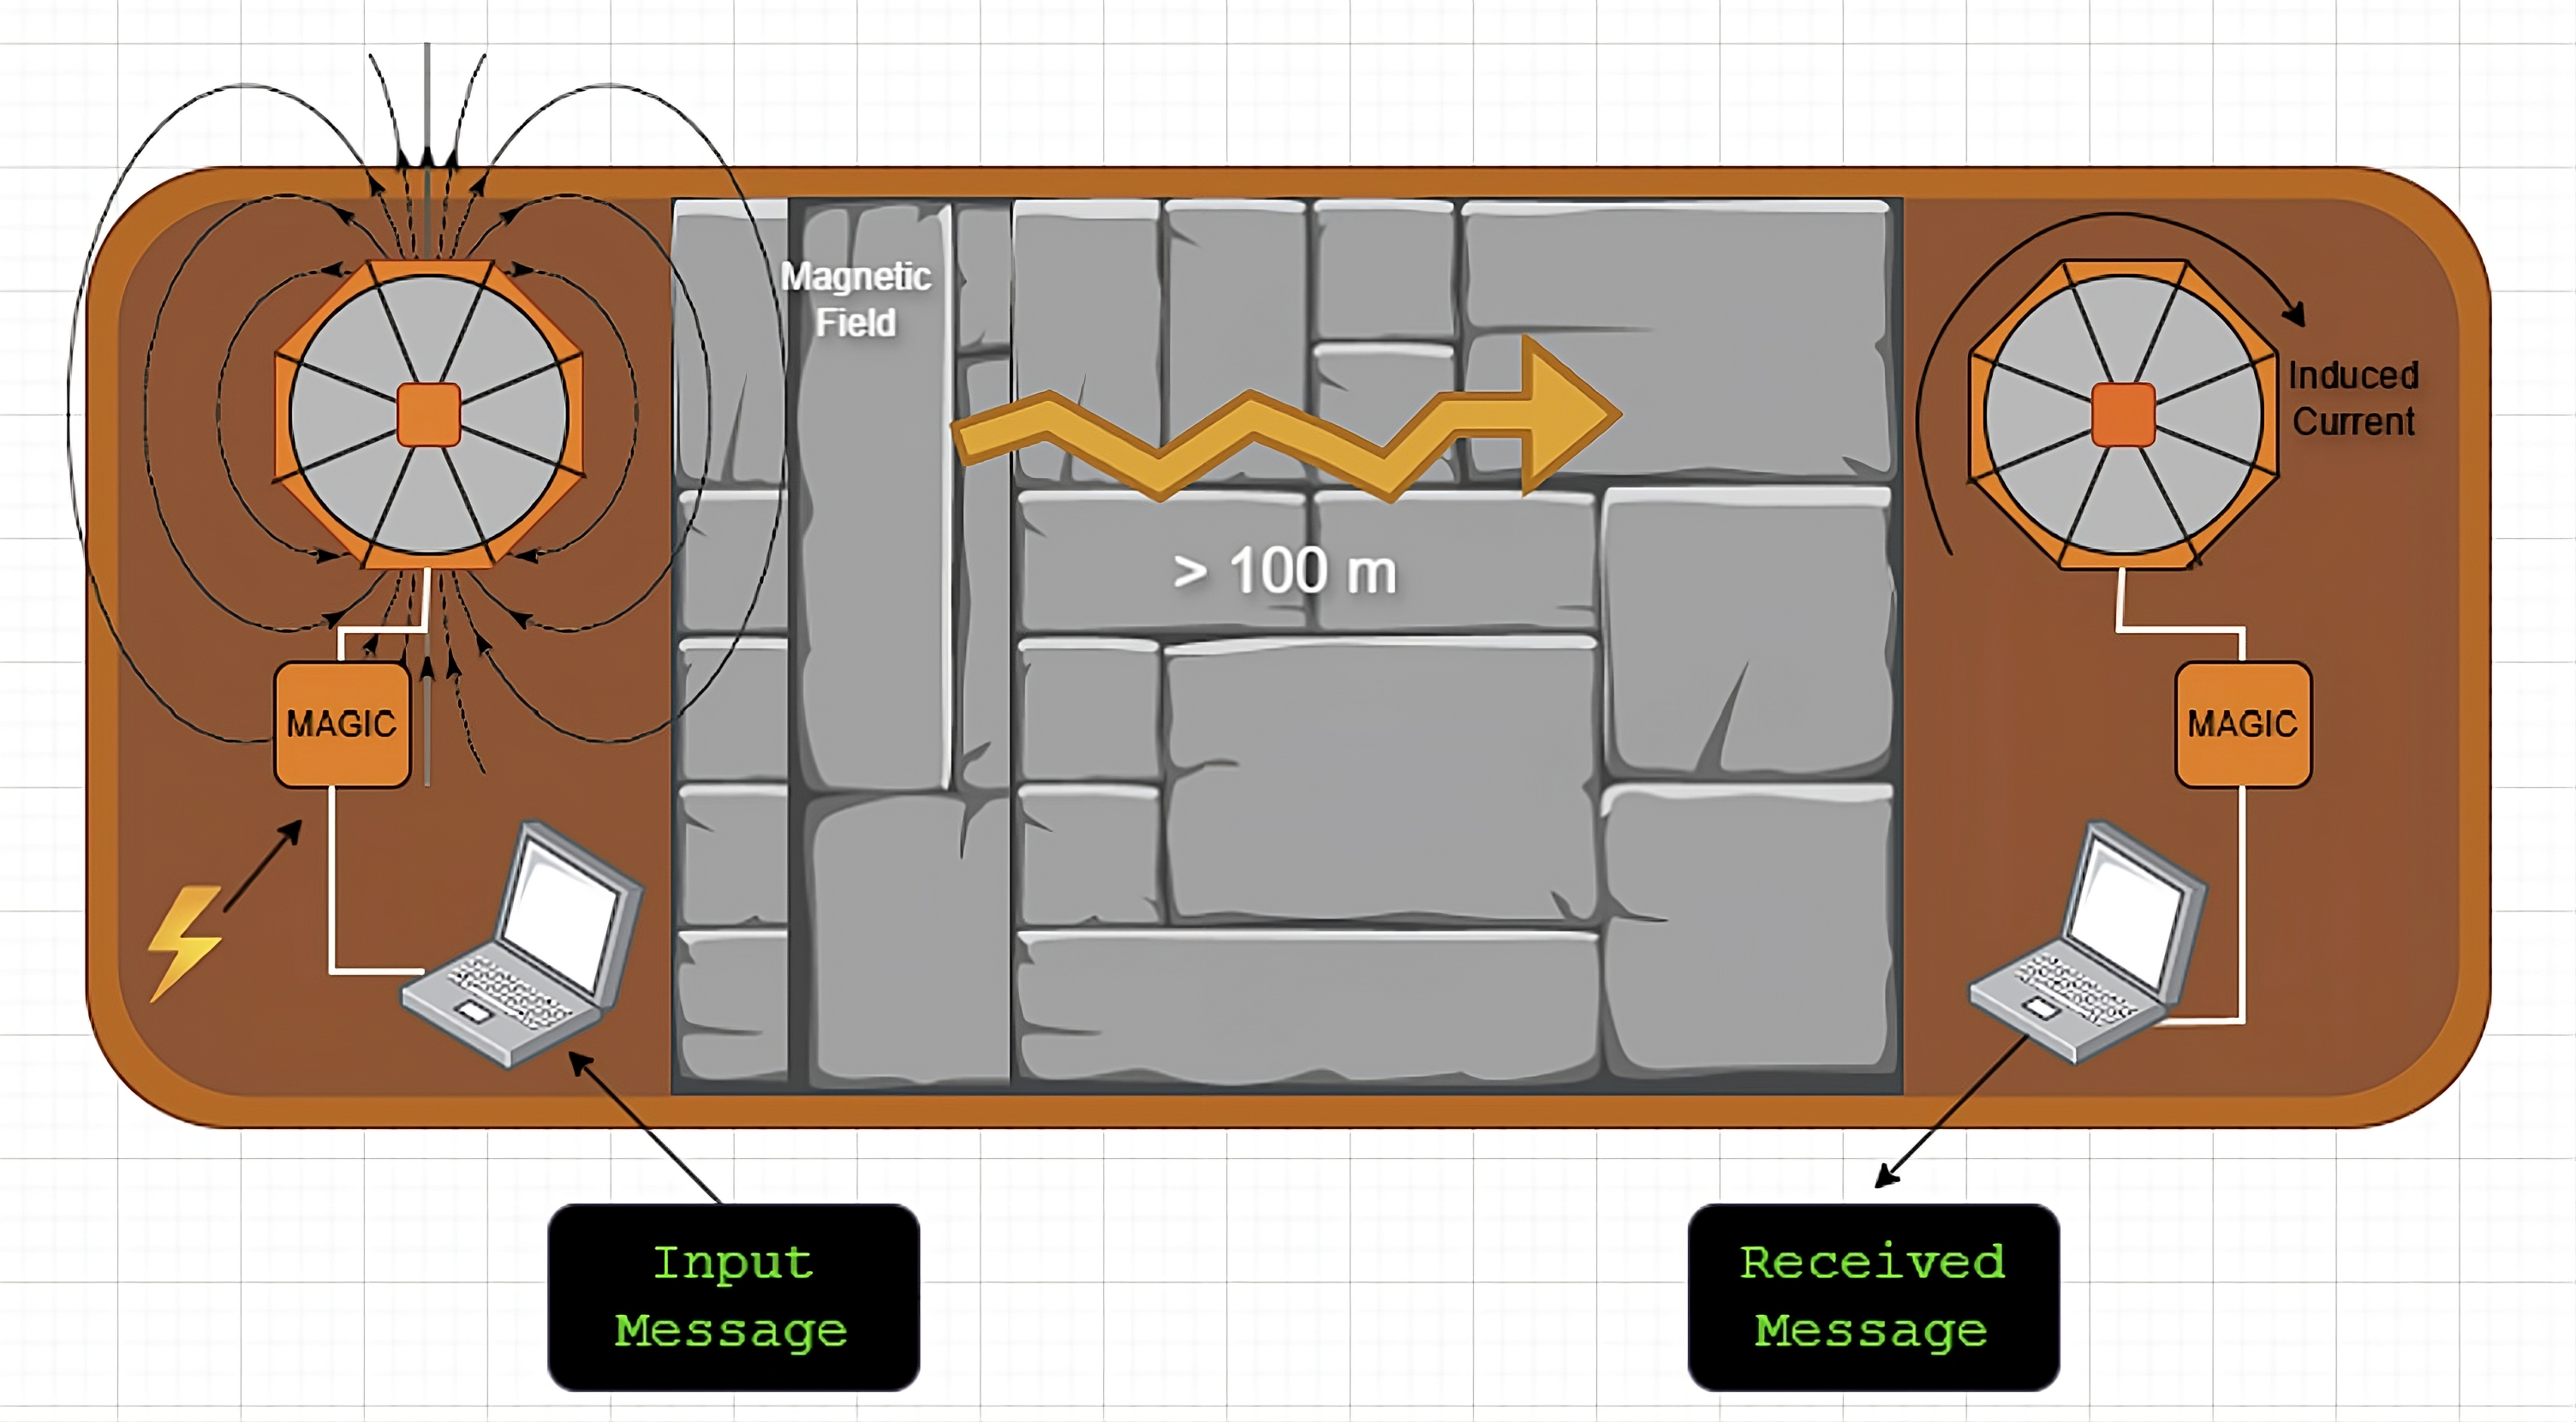
\includegraphics[width=0.8\textwidth]{img/esquema_blanco.png}
    \caption{Conceptual diagram of the complete TTE communication system.}
    \label{fig:system-diagram}

\end{figure}

As shown in the diagram, we can start from left to right with the generation of a text message, wich is codificated and modulated digitally in a computer. Then the digital signal is converted to analog using a DAC, this signal is amplified using a class D audio amplifier to drive the resonant coil. The flux of current at the coil generates a variable magnetic field, as equation \ref{equation_of_ampere_maxwell} describes in section 2. This variable magnetic field, that is centered at a pretty low frequency (VLF band of radio), propagates through the environment, penetrating rock soil and solid material and reaching the receiving coil.
\newp
The magnetic flux that pass perpendicularly through the coil structure can induce a voltage in bornes of the receiving coil, according to Faraday's law of induction \ref{equation_of_magnetic_induction}. This signal can be digitalized using an ADC, demodulated, decoded and corrected in a computer to recover the original text message.
\newp
To answer a received message, the same process is followed in reverse thanks to the switching circuit.
\newp
The schematic diagram of the system is shown in figure \ref{fig:system-schematic}.

\begin{figure}[H]
    \centering
    \includegraphics[width=1\textwidth]{img/schematic.png}
    \caption{Schematic diagram of the complete TTE communication system.}
    \label{fig:system-schematic}
\end{figure}

As is shown in figure \ref{fig:system-schematic}, the system is composed by the following main blocks: Coil (1), Battery (2), USB audio Interface (3) and the core module that contains the Amplifier, a ground loop isolator and the switching Switching circuit(rest of diagram).
\subsection{Coil}
The resonant coil is the element responsible for transmitting the changing magnetic field when current flows through its structure (Transmitter) and for delivering the induced electromotive force (EMF) when the transmitted magnetic field lines pass through its structure (Receiver). To achieve the goal of long-distance communication, the coil must be designed to maximize the efficiency of magnetic energy transfer between the transmitter and receiver. Therefore, a simple toroidal design was initially chosen, where the design and construction variables are reduced to the number of turns (N), the diameter of the structure (D), and the conductor gauge (C). For this first version, the coil diameter was set at 55 cm, as this size was manageable and portable. The conductor gauge was selected based on its cost, electrical resistance, and weight, opting for 17 AWG enamelled copper wire. A table of electrical resistance as a function of conductor gauge, provided by the manufacturer, is shown below.

\begin{table}[H]
    \centering
    \begin{tabular}{|c|c|c|}
    \hline
    \textbf{Gauge (AWG)} & \textbf{Diameter (mm)} & \textbf{Resistance (ohm/m)} \\ \hline
    10                     & 2.588                  & 0.00328                      \\ \hline
    12                     & 2.053                  & 0.00521                      \\ \hline
    14                     & 1.628                  & 0.00829                      \\ \hline
    16                     & 1.291                  & 0.01317                      \\ \hline
    17                     & 1.150                  & 0.01660                      \\ \hline
    18                     & 1.024                  & 0.02100                      \\ \hline
    20                     & 0.812                  & 0.03340                      \\ \hline
    \end{tabular}
    \caption{Electrical resistance as a function of conductor gauge.}
    \label{tab:resistance-table}
\end{table}
%Ajustar valores segun tabla real.

Thus, by choosing this gauge, which corresponds to a diameter of 1.15 mm, and considering a total mass of approximately 1.5 kg, a total length of 156 meters is achieved, which translates to N = 90. With this length, the total resistance of the coil is 2.6 ohms. However, when measured experimentally, the total resistance value is 3 ohms, an ideal value considering the operating resistance of the class D amplifier selected for the project.
\newp
With the geometry and characteristics of the coil defined, the associated electrical parameters are calculated. First, the coil's inductance is calculated using a quick formula for circular coils \cite{utfsm}:

\begin{equation}
    L = \mu*R*N^2*[ln(\frac{8R}{r}) - 2]
\end{equation}
Where:

\begin{itemize}
    \item $L$ is the inductance in Henries (H).
    \item $\mu$ is the permeability of the core (for air, $\mu_0 = 4\pi \times 10^{-7} H/m$).
    \item $N$ is the number of turns.
    \item $R$ is the radius of the coil in meters (m).
    \item $r$ is the radius of the wire in meters (m).
\end{itemize}

Considering an approximate radius $R=0.275$, a conductor radius $r=0.00115$, $N=85$, a theoretical inductance of $L ≈ 13.87mH$ is obtained. However, when measuring the inductance of the constructed coil using an LCR meter, experimental values of $L_1 = 10.67 mH$ and $L_2 = 10.55 mH$ are obtained. This discrepancy can be attributed to factors such as the non-uniform distribution of the magnetic field, conductor losses, and tolerances in the coil's construction.
\newp
At simulations on ANSYS Maxwell, the inductance results in $L \approx 5.7 mH$, a value that is the half of the experimental one, this difference can be explained because in the simulation the wire is considered as an ideal conductor with no thickness, while in the real coil the wire has a diameter of 1.15 mm that affects the magnetic field distribution and the inductance value. %Revisar

\begin{figure}
    \centering
    \includegraphics[width=0.7\textwidth]{img/Maxwell_1.png}
    \caption{Simulation of the magnetic field generated by the resonant coil in ANSYS Maxwell.}
    \label{fig:ansys-coil}
\end{figure}


Finally, the capacitance needed to tune the coil to the desired resonant frequency is calculated, which in this case is 3.2 kHz. The resonant frequency f0 of an LC circuit is given by the formula:
\begin{equation}
    f_0 = \frac{1}{2\pi \sqrt{LC}}
\end{equation}
Solving for the capacitance $C$, we get:
\begin{equation}
    C = \frac{1}{(2\pi f_0)^2 L}
\end{equation}

Thus, the capacitance required to tune the coil to approximately 3.2 kHz results in C ≈ 237 μF for L1 and C ≈ 240 μF for L2. 470 μF ceramic capacitors arranged in series were selected to achieve the desired value, taking into account component tolerances. A diagram of the constructed coil is shown below in figure \ref{fig:coil}.

\begin{figure}[H]
    \centering
    \includegraphics[width=0.5\textwidth]{img/coil.png}
    \caption{Resonant coil constructed for the TTE system.}
    \label{fig:coil}
\end{figure}

\subsection{System characterization}

Knowing the values of inductance and capacitance of the resonant coil, it's possible to characterize the transfer function of the system. Considering the schematic of the induced coupling between two symetrical resonant coils shown in figure \ref{fig:inductive-coupling-schematic}. We can determine the transfer function of the system using the equation described in section 2.3.1.

\begin{figure}
    \centering
    \includegraphics[width=0.5\textwidth]{img/spice.png}
    \caption{Schematic of the inductive coupling between two resonant coils.}
    \label{fig:inductive-coupling-schematic}
\end{figure}

Simulating the system in LTSpice we can obtain the theoretical transfer function of the system, as shown in figure \ref{fig:transfer-function-sim}.

\begin{figure}
    \centering
    \includegraphics[width=0.7\textwidth]{img/spicetf.png}
    \caption{Theoretical transfer function of the resonant coil system.}
    \label{fig:transfer-function-sim}
\end{figure}

For python simulation we obtain a similar result shown in figure \ref{fig:transfer-function-py}.

\begin{figure}
    \centering
    \includegraphics[width=0.7\textwidth]{img/tfpython.png}
    \caption{Theoretical transfer function of the resonant coil system using Python.}
    \label{fig:transfer-function-py}
\end{figure}

When measuring the transfer function for a system where one coil is tuned and another, smaller coil is untuned, as shown in Figure 4.6 for L1 and L2, it can be observed that the resonant frequency is close to 3.2 kHz, fulfilling the initial design.

\begin{figure}[H]
    \centering
    \includegraphics[width=1\textwidth]{img/TF_L1_L2.png}
    \caption{Función de transferencia del sistema de bobinas resonantes.}
    \label{fig:transfer-function}
\end{figure}

The transfer function of the complete system (end-to-end) measured at a distance of 2 meters between the coils is shown below.

\begin{figure}[H]
    \centering
    \begin{subfigure}[b]{0.49\textwidth}
        \centering
        \includegraphics[width=\textwidth]{img/Desfase_end_2_end_2.jpg}
        \caption{Phase shift}
        \label{fig:sub2-transfer-function-system}
    \end{subfigure}
    \hfill
    \begin{subfigure}[b]{0.49\textwidth}
        \centering
        \includegraphics[width=\textwidth]{img/Relacion_de_potencia_end_2_end_3.jpg}
        \caption{Power relation}
        \label{fig:sub1-transfer-function-system}
    \end{subfigure}
    \caption{Transfer function of complete system at 2 meters distance.}
    \label{fig:transfer-function-system}
\end{figure}


If we review particularly the power relation graph in figure \ref{fig:sub1-transfer-function-system} we can observe that the maximum power transfer occurs at a frequency of approximately 3.2 kHz, specifically at 3150 Hz, at this point we have an approximaly analog bandwidth of ~450 Hz considering a decaiment of 3 dB from center frequency. Here it's a zoom of this graph in figure \ref{fig:zoom-transfer-function-system}.

\begin{figure}[H]
    \centering
    \includegraphics[width=0.7\textwidth]{img/bw end-2-end.png}
    \caption{Bandwidth available for end-to-end system at 2 meters distance.}
    \label{fig:zoom-transfer-function-system}

\end{figure}

If we consider this geometry and values of the coil, we can estimate the magnetic field generated at the center of the coil using the formula decribed on section 2 \ref{equation_of_magnetic_field} for the magnetic field at the center of a circular loop:

%ecuacion y calculos pendientes

\subsection{Amplifier and GLI}

The amplifier choosed for the application corresponds to a class D Power Amplifier Board XH-M544  based on the Texas Instruments chips TPA3116D2 and NE5532. This amplifier is capable of delivering a maximum power of 150W Mono, considering a voltage of 26 V.

\newp
This component was selected due to its ability to deliver high power output with high efficiency, which is crucial for driving the resonant coil effectively. The amplifier operates in class D mode, which means it uses pulse-width modulation (PWM) to amplify the input signal, resulting in lower heat dissipation and improved energy efficiency compared to traditional linear amplifiers. %ref pendiente.
Also as was mentioned before, the system will operate in a frequency range around 3.2 kHz, within the audible spectrum. Here is a figure of the amplifier used:

\begin{figure}[H]
    \centering
    \includegraphics[width=0.5\textwidth]{img/amp.png}
    \caption{Amplificador de audio clase D TPA3116D2.}
    \label{fig:amplifier}
\end{figure}

The input signal to the amplifier is provided by a USB audio interface, and this signal is isolated from ground loops using a Ground Loop Isolator (GLI). The GLI is essential to prevent unwanted noise and hum that can be introduced into the audio signal due to differences in ground potential between the computer and the amplifier. By isolating the audio signal, the GLI helps maintain signal integrity and ensures that the transmitted message is clear and free from interference.
%is neccesary if now we utilize a battery?
\newp
Here is a schematic diagram of the GLI used in MAGIC:

\begin{figure}[H]
    \centering
    \includegraphics[width=0.6\textwidth]{img/GLI.png}
    \caption{Schematic diagram of the Ground Loop Isolator (GLI).}
    \label{fig:gli-schematic}
\end{figure}

\subsection{Switching Circuit}
The switching circuit is essential for enabling bidirectional communication in the TTE system, for this prototype this function is supplied by a positional selector, that means, mannually.
\newp
Here is a schematic diagram of the positional selector used MAGIC:.
\begin{figure}[H]
    \centering
    \includegraphics[width=0.8\textwidth]{img/selector.png}
    \caption{Schematic diagram of the switching circuit.}
    \label{fig:switching-circuit}

\end{figure}

This device conmute the bornes of the resonant coil between the amplifier output (TX mode) and the audio interface input (RX mode). When the selector is in position 1, the coil is connected to the amplifier output, allowing it to transmit signals. Conversely, when the selector is in position 2, the coil is connected to the audio interface input, enabling it to receive signals. Also the selector at TX mode allows the amplifier to be powered on.

 

\subsection{Audio Interface}

The audio interface selected for the TTE communication system is the SoundBlaster Play! 3 by Creative Labs. This USB audio interface is chosen for its high-quality audio conversion capabilities, compact size, input and output separately channel and ease of use. In terms of USB audio interfaces, the SoundBlaster Play! was the best option available considering cost and Portability.
\newp
Here is a figure of the audio interface used:
\begin{figure}[H]
    \centering
    \includegraphics[width=0.3\textwidth]{img/sbp3.png}
    \caption{USB Audio Interface SoundBlaster Play! 3.}
    \label{fig:audio-interface}
\end{figure}

\subsection{Additional Components and considerations}

The whole system is powered by a 24V Li-ion battery pack, providing sufficient voltage and current to drive the amplifier and other components. The use of a battery pack ensures portability and allows the system to operate in remote locations without access to mains power. The battery can provide 27 V at maximum charge, which is abive the operational voltage of the amplifier, generating interruptions in transmission, so a buck converter $XH-M400$ is used to regulate the voltage to a stable 24 V output.
\begin{figure}
    \centering
    \includegraphics[width=0.5\textwidth]{img/battery_and_buck.png}
    \caption{24V Li-ion Battery Pack and Buck Converter.}
    \label{fig:battery}
\end{figure}

This componens were packaging in addition with a switch and DC connectors in a 3D printed enclosure designed and printed for this specific purpose. Here is a figure of the result:

\begin{figure}
    \centering
    \includegraphics[width=0.5\textwidth]{img/Ensamblaje_bat.jpg}
    \caption{3D printed enclosure for the core module of MAGIC.}
    \label{fig:enclosure}
\end{figure}
%incluir también imagenes reales de la construcción

The rest of the components that are not marked in the schematic diagram on figure \ref{fig:system-schematic} are also enclosed in another 3D printed box, denominated core module of MAGIC, that contains the amplifier, GLI, positional selector and a voltimeter/amperimeter monitor. This module is connected to the coil due to typical DC connector and the audio interface using standard audio cables with 3.5 mm jacks.

\begin{figure}
    \centering
    \includegraphics[width=0.5\textwidth]{img/Ensamblaje_case_MAGIC_V1.jpg}
    \caption{Core module of MAGIC communication system.}
    \label{fig:core-module}
\end{figure}

Other pieces were designed and printed in 3D to support the coil, the conductors over the structure and to protect the capacitor bank. Here is a figure of these pieces:

%Figura pendiente

Finally the whole system is presented in figure \ref{fig:complete-system}.

\begin{figure}[H]
    \centering
    \includegraphics[width=0.7\textwidth]{img/MAGIC_complete_system.png}
    \caption{Complete TTE communication system MAGIC.}
    \label{fig:complete-system}
\end{figure}

\section{Software Developement}


%Actualizar imagen con la batería

\subsection{Design}
The software component of the TTE communication system is responsible for coding, modulate and generate the message signal at the Transmitter, and filter, detect, demodulate, and decode the recewived signals at the receiver. The software is developed in Python, leveraging libraries such as NumPy and SciPy for signal processing tasks.
\newp
The modulation scheme selected for the system is non-coherent Frequency Shift Keying (FSK). This choice is motivated due to its robustness to phase variations. As it was explain in Chapter II, the composition of the media can produce significant phase shifts and frequency offsets that can affect the performance of coherent modulation schemes, in fact the magnetic coupling scheme is intrinsically dispersive at resonant frequency and that goes even worse when the constant of coupling $k$ is reduced by the distance and other attenuation sources.

\subsection {Transmitter}

The transmitter software is responsible for converting the text message into a modulated signal suitable for transmission via the resonant coil. The process involves several key steps:

\subsubsection{Message coding and modulation}

the function of MAGIC is generate a text message link so is necessary to generate in principe any letter of the alphabet and all the numbers, if we consider also other characters like punctuation marks and special symbols, the quantity o different characters to code increase significantly. In that way we can use the ASCII (American Standard Code for Information Interchange) coding scheme, that has 128 different characters.
\newp
To encode characters using FSK modulation, we can assign a unique frequency to each character. However, this means that we need at least 128 different frequencies in our constellation and also we have to consider a minimum spectral separation between tones to achieve the ortogonallity condition. This requirement can lead to a very wide bandwidth, and we want to concentrate the constellation at the center frequency of the resonant coil in order to favor the conditions of communication.
\newp
To address this challenge, we can implement a multi-level FSK scheme, where each symbol represents multiple bits of information. For example, if we use 16 different frequencies, each symbol can represent 4 bits (since $2^4 = 16$). If we use a combination of two symbols per character, we can represent 8 bits (1 byte) per character, which is enough to cover the entire ASCII set. Actually we can use the extended ASCII table that has 256 characters.
\newp
For example the character 'A' has an ASCII value of 65, we can obtain two hexadecimal digits from this value: 4 and 1, that corresponds to the integer division and the module of the original value and 16, then we transform the hexadecimal digits to its decimal form and map to the corresponding FSK frequency. In this case 4 maps to $f4$ and 1 maps to $f1$.

\subsubsection{Ortogonality and Bandwidth}

As mentioned in previous chapters, carrier orthogonality is a crucial aspect of FSK modulation systems, ensuring that signals transmitted at different frequencies do not interfere with each other. In other words, the energy of a symbol transmitted at a given frequency does not enter the spectral channel of an adjacent symbol within the symbol constellation. For orthogonality to be met, the relationship between the sampling frequency and the number of samples per symbol must be considered; that is, the inverse of the duration of each symbol. The relationship between the carrier frequencies f1 and f2 must satisfy the following equation:

\begin{equation}
    f_2 - f_1 = \frac{k}{T_s} = \frac{k f_s}{N_s}
\end{equation}

In this case, the sampling frequency is 48 kHz, and the number of samples per symbol, Ns, must be defined. To determine the optimal value of Ns, several tests were performed varying this parameter and observing its impact on the demodulated symbol error rate (SER) of the system. The variation of SER as a function of symbol length for a defined SNR value is shown below. This SNR corresponds to the minimum target to be achieved with the TTE communication system; in this case, $SNR = −10 dB$. %detallar luego el criterio para cálculo de SNR (en la banda, qué banda) .

\begin{figure}[H]
    \centering
    \includegraphics[width=0.7\textwidth]{img/SER_vs_Ns.png}
    \caption{SER vs Ns for 8-FSK and 16-FSK at SNR = -10 dB.}
    \label{fig:SER-vs-Ns}
\end{figure}

Considering a bandwidth of 200 Hz, a symbol length of 24000 is an ideal value for 8 and 16 FSK models. The point marked with a red dotted line in Figure \ref{fig:SER-vs-Ns} indicates an error rate of approximately 12\% for 16 symbols and 5\% for eight symbols. For both models, this error level is acceptable considering that a simple error correction code will be included later. This symbol length is chosen over a longer one that could further decrease the SER because the system's data rate is not to be sacrificed excessively, maintaining a suitable balance between transmission speed and noise robustness. Having thus set the value of Ns = 24000, the separation between the carrier frequencies is calculated to meet the orthogonality condition. Considering k = 1, the minimum separation between carriers is 2 Hz, however, given that the FFT resolution in the demodulator depends on the number of samples per symbol, a larger separation is selected, leaving spectral channels unused to avoid interference between adjacent symbols. Later, the difference in performance will be observed when considering a single-channel demodulation model and taking the maximum separation between the channel of the expected symbol and its adjacent symbols.

\subsubsection{Constellation of frequencies}

Once we have defined the number of symbols to use and the minimum frequency separation to achieve orthogonality, we can proceed to define the frequency constellation for the FSK modulation.
\newp
At the beggining we define the 16 frequencies around the center frequency of the system that corresponds approximately to 3.2 kHz. Considering a minimum separation of 4 Hz, thats because we want to leave a spectral channel between symbols considering the FFT resolution at the demodulator. With this criteria we can use a minimum bandwidth of 60 Hz to allocate the 16 frequencies.

\begin{figure}[H]
    \centering
    \includegraphics[width=0.7\textwidth]{img/constellation_old.jpg}
    \caption{Frequency constellation for 16-FSK modulation.}
    \label{fig:frequency-constellation}
\end{figure}

In figure \ref{fig:frequency-constellation} we can observe the defined frequency constellation for the 16-FSK modulation scheme and a measure o  the spectrum of noise in one of the locations where the system was tested in Cerro Calán. The noise, that is also, filtered by a digital filter shows an electrical grid harmonic at 3150 Hz, that is close to the first symbol frequency.
\newp
After doing several measurements of teh spectral distribution of Noise in different locations, it was observed that the odd harmonics of the electrical grid (i.e., 3150 Hz, 3250 Hz, etc.) were really prominent, while the even harmonics were less significant. Here are some examples of noise spectrums measured in different locations.

\begin{figure}[H]
    \centering
    \begin{subfigure}[b]{0.49\textwidth}
        \centering
        \includegraphics[width=\textwidth]{img/100m 200m and noise/power_spectrum_density_of_noise_at_calicata.png}
        \caption{Two measurements of noise at Calicata in Cerro Calán.}
        \label{fig:noise-spectrum-1}
    \end{subfigure}
    \hfill
    \begin{subfigure}[b]{0.49\textwidth}
        \centering
        \includegraphics[width=\textwidth]{img/100m 200m and noise/power_spectrum_density_of_noise_at_copa.png}
        \caption{Two measurements of noise at Copa in Cerro Calán.}
        \label{fig:noise-spectrum-2}
    \end{subfigure}
    
    \vspace{1em} % Add some vertical space between rows

    \begin{subfigure}[b]{0.49\textwidth}
        \centering
        \includegraphics[width=\textwidth]{img/100m 200m and noise/power_spectrum_density_of_noise_at_lab.png}
        \caption{Two measurements of noise at Millimeter Wave Laboratory in Cerro Calán.}
        \label{fig:noise-spectrum-3}
    \end{subfigure}
    \hfill
    \begin{subfigure}[b]{0.49\textwidth}
        \centering
        \includegraphics[width=\textwidth]{img/100m 200m and noise/DB Selec.png}
        \caption{Noise at Gautier.}
        \label{fig:noise-spectrum-4}
    \end{subfigure}
    \caption{Noise spectrum measurements at different locations in Cerro Calán.}
    \label{fig:noise-spectrums}
\end{figure}

Here is the noise spectral density measured at different locations in Cerro Calán, combined:

\begin{figure}[H]
    \centering
    \includegraphics[width=1\textwidth]{img/100m 200m and noise/Ruido dB scale.png}
    \caption{Combined noise spectrum from different locations in Cerro Calán.}
    \label{fig:combined-noise-spectrum}
\end{figure}


Although the even electricac grid harmonics are strangely less significant, to avoid potential interference, the frequency constellation was designed to avoid these harmonics as well. Therefore, the selected frequencies for the FSK modulation scheme was modified, defining flagged bands without symbols around both odd and even harmonics. Here is the final frequency constellation used in the system:


\begin{table}
    \centering
    \begin{tabular}{|c|c|}
    \hline
    \textbf{Symbol} & \textbf{Frequency (Hz)} \\ \hline
    0               & 3136                    \\ \hline
    1               & 3164                    \\ \hline
    2               & 3168                    \\ \hline
    3               & 3172                    \\ \hline
    4               & 3176                    \\ \hline
    5               & 3180                    \\ \hline
    6               & 3184                    \\ \hline
    7               & 3188                    \\ \hline
    8               & 3212                    \\ \hline
    9               & 3216                    \\ \hline
    A               & 3220                    \\ \hline
    B               & 3224                    \\ \hline
    C               & 3228                    \\ \hline
    D               & 3232                    \\ \hline
    E               & 3236                    \\ \hline
    F               & 3264                    \\ \hline
    \end{tabular}
    \caption{Final frequency constellation for 16-FSK modulation.}
    \label{tab:final-frequency-constellation}
\end{table}

As result here is a spectrum of noise with the frequency symbols marked:

\begin{figure}[H]
    \centering
    \includegraphics[width=1\textwidth]{img/100m 200m and noise/new constellation.png}
    \caption{Final frequency constellation over noise spectrum.}
    \label{fig:final-constellation-with-noise}
\end{figure}


\subsection{Receiver}

 The detection system works as a typical non-coherent FSK receiver. The data is aquired using an ADC at a sample rate of 48 kHz, then the digital signal is processed in real-time to determine when the message is coming. The main steps of the receiver algorithm are filtering, correlation, demodulation and decoding. 

%is there any best way of describing this? What are the others benefits of filtering the signas with a digital bandpassfilter,if are any ?

\newp
In comparisson for example models based on PSK or QAM, that are more sensitive to phase noise and frequency offsets. FSK modulation allows the receiver to detect the transmitted symbols based on energy detection in specific frequency bands, without requiring precise phase synchronization. This characteristic makes non-coherent FSK particularly suitable for TTE communication systems, where the channel conditions can be highly variable and unpredictable.
Here is a diagram of the receiver algorithm \ref{fig:fsk-mod-demod}.

\begin{figure}[H]
    \centering
    \includegraphics[width=0.8\textwidth]{img/Diagrama_Receptor.png}
    \caption{Block diagram of the non-coherent FSK modulation and demodulation process.}
    \label{fig:fsk-mod-demod}
\end{figure}

At the beggining the digital signal is filtered and then passes to a Window of len N, that is an important number, the dimensions of this Window determine the cost of the main process of detection, that's mean, the IQ correlation. The bigger the window is, more calculations occurred in each earing cycle.
\newp
The data present con window is processed using the correlation by parts algorithm, that is explained in the next section. The output of this process is an array of correlation, in wich we can obtain the maximum, if this peak of correlation is above a certain threshold, thats is previously determined by the place conditions, we save that value and their position. If not, we discard the time older data chunk to put a new one. That's why the window is also a queue structure, specifically a \textit{deque} from the collections library of python.
\newp
If we have detected a peak of correlation, we repeat the process saving the peaks and their position in the next earing cycles, when the peak is identified as a global one, achieving a increase and then a decrease in its value, we proceed to save the data that temporally is next from preamble, that's is, counting samples from the position of the peak plus the size of the preamble. Once the message position is known, proceeds to save the following symbols knowing beforehand the size of the total message.
\newp
The demodulation process is performed by calculating the FFT of each symbol received and determining which frequency has the highest energy. This frequency is then mapped back to the corresponding symbol in the FSK constellation. Finally, the decoded symbols are converted back into characters using the inverse of the encoding scheme used at the transmitter. Also parity symbols anre checked to correct possible errors in the received message.

\subsubsection{Digital Filter}

The digital filter used in the receiver is a bandpass filter designed to isolate the frequency band of interest around the FSK symbol frequencies while attenuating noise and interference outside this band. The filter is implemented using butterworth design due to its maximally flat frequency response in the passband, which helps preserve the integrity of the received signal. for this design we use the scipy function \textit{buttord} to define the performance and frequency response of the filter and \textit{butter} to create the filter coefficients. The specifications are:

\begin{itemize}
    \item Passband frequencies: 3130 Hz to 3270 Hz
    \item Stopband frequencies: 3110 Hz and 3290 Hz
    \item Passband loss: 1 dB
    \item Stopband attenuation: 40 dB
\end{itemize}

The filter is applied with function \textit{filtfilt} from scipy library, that performs zero-phase filtering by processing the input signal in both the forward and reverse directions. This approach helps to eliminate phase distortion introduced by the filter, which is particularly important in communication systems where phase information can be critical for accurate symbol detection.%cita pendiente
\newp
Here is the frequency response of the designed bandpass filter:

\begin{figure}[H]
    \centering
    \includegraphics[width=0.7\textwidth]{img/Respuesta_filtro.png}
    \caption{Frequency response of the designed bandpass filter.}
    \label{fig:filter-response}
\end{figure}

\subsubsection{Correlation Process}

Correlation is a mathematical operation that measures the similarity between two signals as a function of the time-lag applied to one of them %Include Bibliography. 
In the context of signal processing, correlation is often used to detect the presence of a known signal (template) within a received signal that may be corrupted by noise.
In the non-coherent FSK detection system, the correlation process is used to compare the received signal with predefined reference signals corresponding to each of the FSK frequencies. 
The correlation here is performs between the received signal (or a portion of it) and a known preamble.
This preamble is a specific sequence of symbols that is transmitted at the beginning of each data packet. The purpose of the preamble is to help the receiver synchronize with the incoming signal and accurately detect the start of the data transmission. %Include Reference)
Here we have several main design parameters: an optimar lenght of preamble, its structure, and optimal use of our computation resources, thats because as bigger the lenght of correlation inputs, more calculus to do in each earing time. %Improve redaction
The size of the window is key of the times that the function \textit{Correlation by parts} is called. 
The output of the correlation process is a correlation coefficient that indicates the degree of similarity between the received signal and the reference signal at different time lags. A high correlation coefficient at a specific time lag suggests that the known signal is present in the received signal at that time.
% Include bibliography
The correlation formula (\ref{eq:Correlation_dig}), given in previous chapter, is used as a the main operation of correlation IQ System.



\subsubsubsection{Correlation by parts algorithm}

The correlation by parts algorithm is a method to efficiently compute the correlation between a received signal and the known parts of the preamble considering the similarity with in phase and cuadrature tones.
\newp
At the beggining we have a window of size $N_w$, wich is the size of the total preamble ($N_symbols$ multiplied by the size of each symbol $M$), plus the amount of samples incoming in an earing cicle ($N_c$). With this structure we allow only one instance of correlation where the incoming preamble is fully contained in the window. So from the window we can define $N_symbols$ parts, where each part $S_N$ corresponds to the section that could contain te $``N"th$ symbol of the preamble.
\newp
once we have the $S_N$ and $P_N$ (the $``N"th$ symbol of the preamble) we can compute the correlation between them using the formula (\ref{eq:Correlation_dig}). That is implemented as the scipy function \textit{correlate} with mode ``valid", that has an output size of the difference between the two arguments ($S_N - P_N$). For each of these $``N"$ calculus The $S_N$ signals are correlated with its corresponding $P_N$ symbol of and its version in cuadrature, that means the following:

\begin{equation}
\label{eq:corr_IQ}
\begin{split}
    I_{N} &= \sum_{k=0}^{M-1} S_{N}[k] \sin(2 \pi f_{N} k T_s) \\
    Q_{N} &= \sum_{k=0}^{M-1} S_{N}[k] \cos(2 \pi f_{N} k T_s)
\end{split}
\end{equation}

where $f_N$ is the frequency of the $``N"th$ symbol of the preamble and $T_s$ is the sampling period.
\newp

So at the output we have two arrays that represents the similarity of the incoming signal section with the correspondig symbol in phase and cuadrature. If we consider the totallity of operations we can define two Matrix I and Q of size $N_symbols$ x $n_c$, where each row corresponds to the arrays resulted in \ref{eq:corr_IQ}:

\begin{equation}
\label{eq:matrix_IQ}
    I = \begin{bmatrix}
    I_{1}[0] & I_{1}[1] & \dots & I_{1}[n_c-1] \\
    I_{2}[0] & I_{2}[1] & \dots & I_{2}[n_c-1] \\
    \vdots & \vdots & \ddots & \vdots \\
    I_{N}[0] & I_{N}[1] & \dots & I_{N}[n_c-1]
    \end{bmatrix}, \quad
    Q = \begin{bmatrix}
    Q_{1}[0] & Q_{1}[1] & \dots & Q_{1}[n_c-1] \\
    Q_{2}[0] & Q_{2}[1] & \dots & Q_{2}[n_c-1] \\
    \vdots & \vdots & \ddots & \vdots \\
    Q_{N}[0] & Q_{N}[1] & \dots & Q_{N}[n_c-1]
    \end{bmatrix}
\end{equation}

Then we take the absolut value of each element of the two matrix and sum them to obtain a final correlation matrix C:

\begin{equation}
\label{eq:final_correlation_matrix}
    C = \begin{bmatrix}
    |I_{1}[0]| + |Q_{1}[0]| & |I_{1}[1]| + |Q_{1}[1]| & \dots & |I_{1}[n_c-1]| + |Q_{1}[n_c-1]| \\
    |I_{2}[0]| + |Q_{2}[0]| & |I_{2}[1]| + |Q_{2}[1]| & \dots & |I_{2}[n_c-1]| + |Q_{2}[n_c-1]| \\
    \vdots & \vdots & \ddots & \vdots \\
    |I_{N}[0]| + |Q_{N}[0]| & |I_{N}[1]| + |Q_{N}[1]| & \dots & |I_{N}[n_c-1]| + |Q_{N}[n_c-1]|
    \end{bmatrix}
\end{equation}

So in the components of this last matrix we have a certain measure about similarity between the incoming signal sections and the preamble symbols, in every columns there is an intant of time so if we sum along the rows we can obtain a final correlation vector that indicates the total similarity between the incoming signal and the whole preamble at each instant of time:
\begin{equation}
\label{eq:final_correlation_vector}
    V = \begin{bmatrix}
    \sum_{n=1}^{N} C_{n}[0] & \sum_{n=1}^{N} C_{n}[1] & \dots & \sum_{n=1}^{N} C_{n}[n_c-1]
    \end{bmatrix}
\end{equation}

As result we can see something like this:

\begin{figure}[H]
    \centering
    \includegraphics[width=0.7\textwidth]{img/Simulacion corr IQ.png}
    \caption{Resulted Correlation by parts with 24 symbols preamble.}
    \label{fig:corr-by-parts-diagram}
\end{figure}

\subsubsection{Demodulation and Decoding}

The demodulation process occurs ``offline" once the preamble is detected and the message symbols are extracted from the received signal. Each symbol is processed individually to determine which frequency was transmitted.
\newp
For each symbol, the FFT is computed to analyze its frequency content. The resolution of the FFT is determined by the number of samples in each symbol, which is 24000 in this case. This provides a quantity of spectral bins of 12000, that's because the FFT of a real-valued signal is symmetric, so we only need to consider the first half of the spectrum, that is distributed from 0 Hz to 24 kHz, the Nyquist frequency.
\newp
We proofed two demodulation schemes: single channel and multi channel. In the single channel demodulation, we simply identify the frequency bin with the highest magnitude between the spectral channels corresponding to the defined FSK frequencies. In multi channel demodulation, we consider not only the magnitude of the expected frequency bin but also the magnitudes of its adjacent bins, considering a weighted sum to determine the transmitted symbol.

\begin{figure}
    \centering
    \includegraphics[width=1\textwidth]{img/100m 200m and noise/candidate def.png}
    \caption{Example of spectrum.}
    \label{fig:demodulation-schemes}
\end{figure}

In the figure \ref{fig:demodulation-schemes} we can observe an example of the spectrum of a received symbol. In this case, the expected frequency bin corresponds to symbol '5' at 3180 Hz. In single channel demodulation, we would simply select this bin as the detected symbol. This capture of demodulation was a real communication test at 200 meters of distance.



\subsubsection{Correction Error Code}

The error correction code implemented in the TTE communication system is based on Reed-Solomon coding, which is a block code capable of correcting multiple symbol errors within a codeword. Reed-Solomon codes are particularly well-suited for applications where burst errors are common, as they can correct errors that affect multiple consecutive symbols.
\newp
The implementation utilizes the RSCodec class from the $reedsolo$ library \cite{pypiClientChallenge}, which provides a convenient interface for encoding and decoding messages using Reed-Solomon codes. We have to take in mind that this code work at a bytes level, so the parity symbols added are actually pairs of symbols in base 16. 
\newp
Since MAGIC's character base also has 256 possible values, the encoding requires two contiguous symbols (in base 16) to form a byte. Thus, Reed Solomon can correct X/2 bytes if X parity bytes are defined. Since each byte consists of 2 symbols in base 16, 4 parity symbols are needed to fix a character. Because each character is composed of 2 symbols, the implemented model does not have the "granularity" to correct each symbol individually, but instead pairs of them.

In this way, if, for example, 20 parity symbols are defined, 5 characters can be corrected, regardless of whether these characters are corrupted by one or both of the symbols that compose them.

\subsection{Preamble design}

As explained in the design of the message reception and detection system, the preamble plays a crucial role in the synchronization and subsequent demodulation of the transmitted symbols. The preamble must be carefully designed to maximize the probability of detection in the presence of noise and other channel distortions.
\newp
Therefore, a computationally generated sequence of random symbols, known to both the transmitter and the receiver, was chosen. This sequence must be long enough to provide a clear reference for detection, but not so long as to consume excessive transmission time. A total preamble length of 12 seconds was then defined. This value was determined through months of testing at different communication distances in underground environments.
\newp
As long as the peak correlation was visible under the project's target communication conditions, there was no limit to its duration. This particular preamble length is the result of the trade-off between detection probability and an acceptable transmission time for the application.
\newp
The following shows the piecewise correlation results for different preamble structures, considering a total length of 12 seconds.

\begin{figure}
    \centering
    \label{fig:preamble-corr-models}
    \includegraphics[width=1\textwidth]{img/Simulacion corr modelos_2.png}
    \caption{Correlation by parts for different preamble structures with 12 seconds length.}
\end{figure}

Some relevant data about this excersice is summarized in the following table:
\newp

\begin{tabular}{|l|l|l|l|l|l|l|}
\hline N & M & Max Peak & Std Noise & Mean Noise & Ratio & Time (s) \\
\hline 3 & 192000 & $4.00 \mathrm{e}+05$ & 4842.85 & 14029.95 & 16.86 & 0.81 \\
\hline 6 & 96000 & $4.04 \mathrm{e}+05$ & 6141.66 & 22835.93 & 11.5 & 1.47 \\
\hline 12 & 48000 & $4.19 \mathrm{e}+05$ & 4233.53 & 33777.56 & 9.91 & 2.58 \\
\hline 24 & 24000 & $4.09 \mathrm{e}+05$ & 5155.71 & 48747.34 & 6.92 & 5.71 \\
\hline 48 & 12000 & $4.05 \mathrm{e}+05$ & 4506.15 & 69383.46 & 5.17 & 13.72 \\
\hline
\end{tabular}

The figure \ref{fig:preamble-corr-models}
shows that while the IQ correlation level is similar for each preamble topology considered, as the number of symbols in the sequence increases, the correlation peak becomes "thinner," meaning it is concentrated in a smaller number of earing moments. This is beneficial for the detection system, as it allows for more precise identification of the start of the transmitted message.



\subsection{Decimation?}

The inclusion of a decimation process in the system's reception stage was evaluated, aiming to reduce the amount of data to be processed and thereby decrease the computation time required for message demodulation. 
\newp
Decimation, as explained in Section 2, consists of reducing the sampling rate of the received signal while maintaining the essential information for detection and demodulation. The decimation process was implemented by evaluating two stages of filtering and downsampling. In the first stage, a digital bandpass filter operating between 3100 and 3300 Hz was applied, followed by downsampling by a factor of 12. It is essential to note that when considering this decimation factor, the Nyquist frequency of the resulting system is 4000 Hz; therefore, the recoverable zones are found every 2000 Hz. For this first case, the second Nyquist zone is taken, considering the interval between 2000 and 4000 Hz. The bandpass filter must eliminate all components outside this range to avoid aliasing.
\newp
In the second stage, a bandpass filter is applied between 700 and 900 Hz, followed by downsampling by a factor of 4. In this case, the Nyquist frequency of the resulting system is 1000 Hz; therefore, the second zone, between 500 and 1000 Hz, is again selected. Once more, the bandpass filter is within this window, suppressing components outside this range to avoid aliasing.
\newp
This reduces the sampling rate of the original 48 kHz system to a final rate of 1000 Hz, representing a significant reduction in the amount of data to be processed.

\begin{figure}
    \centering
    \includegraphics[width=0.7\textwidth]{img/decimacion/filters_decimation.png}
    \caption{Decimation filters applied in decimation process.}
    \label{fig:decimation-process}
\end{figure}

%Incluir diagrama de la elección de zonas de Nyquist y filtros aplicados.


\newp
While the decimation process reduces the amount of data to be processed, multiple field tests have shown that the variability of the correlation peak increases with this process, making it difficult to detect the start of the transmitted message accurately. 
\newp
The following measurement, taken with a direct connection (via cable) between the transmitter and receiver, evaluates the variability of the correlation peak when the decimation process is applied compared to the system without decimation.

\begin{figure}[H]
    \centering
    \begin{subfigure}[b]{0.49\textwidth}
        \centering
        \includegraphics[width=\textwidth]{img/decimacion/Correlation_64_symbols_NW.png}
        \caption{Correlation form Signal 64 symbols without decimation.}
        \label{fig:64_NW}
    \end{subfigure}
    \hfill
    \begin{subfigure}[b]{0.49\textwidth}
        \centering
        \includegraphics[width=\textwidth]{img/decimacion/Correlation_64_symbols_NW_ D.png}
        \caption{Correlation form Signal 64 symbols with decimation.}
        \label{fig:64_NW_D}
    \end{subfigure}
    
    \vspace{1em} % Add some vertical space between rows

    \begin{subfigure}[b]{0.49\textwidth}
        \centering
        \includegraphics[width=\textwidth]{img/decimacion/Correlation_128_symbols_NW.png}
        \caption{Correlation form Signal 128 symbols without decimation.}
        \label{fig:128_NW}
    \end{subfigure}
    \hfill
    \begin{subfigure}[b]{0.49\textwidth}
        \centering
        \includegraphics[width=\textwidth]{img/decimacion/Correlation_128_symbols_NW_D.png}
        \caption{Correlation form Signal 128 symbols with decimation.}
        \label{fig:128_NW_D}
    \end{subfigure}
    \caption{Correlation form Signal with and without decimation for signals with 64 and 128 symbols.}
    \label{fig:corr-peak-variability}
\end{figure}

In principe the form of the simple correlation is similar in both cases, however, when analyzing the variability of the peak of correlation over multiple measurements, it is observed that when the data is decimated, the variability increase:

\begin{figure}
    \centering
    \begin{subfigure}[b]{0.8\textwidth}
        \includegraphics[width=\textwidth]{img/decimacion/Power_and_xcorr_64_nw.png}
        \caption{Variability of correlation at model signal 1.}
        \label{fig:correlation-peak-variability-no-decimation}
    \end{subfigure}
    
    \vspace{1em} % Add some vertical space between rows
    
    \begin{subfigure}[b]{0.8\textwidth}
        \centering
        \includegraphics[width=\textwidth]{img/decimacion/Power_and_xcorr_64_nw.png}
        \caption{Variability of correlation peak at model signal 2.}
        \label{fig:correlation-peak-variability-decimation}
    \end{subfigure}
    \caption{Variability of correlation peak with and without decimation.}
    \label{fig:correlation-peak-variability-graph}
\end{figure}

It's clear that for both signals the variability of the peak of correlation is significantly higher when the decimation process is applied. This increased variability generates a lot of cases of no detection of the preamble, which is unacceptable for the system's operation. That's why MAGIC's final design does not include the decimation process in the reception stage.


\section{Testing and Validation}

During the development of the TTE communication system, multiple tests were conducted to evaluate its performance in various scenarios. These tests aimed to validate the design choices made and to assess the system's ability to operate effectively in real-world conditions. The following subsections detail the different testing scenarios, results obtained and some other tests.

\subsection{Induction Pattern}
 The decaiment of the power available in the reeiver coil as a function of the relative angle between coils was measure at surface level in a open field. The transmitter coil was fixed in a horizontal position, while the receiver coil was rotated in steps of 5$\degree$ 
from -45$\degree$ to 45$\degree$ considering 0$\degree$ when coils are perfectly aligned.
\begin{figure}
    \centering
    \begin{subfigure}[b]{0.49\textwidth}
        \centering
        \includegraphics[width=\textwidth]{img/MAGIC_PI.png}
        \caption{Setup for transmitter.}
        \label{fig:induction-pattern-TX}
    \end{subfigure}
    \hfill
    \begin{subfigure}[b]{0.49\textwidth}
        \centering
        \includegraphics[width=\textwidth]{img/MAGIC PI 2.png}
        \caption{Setup for receiver.}
        \label{fig:induction-pattern-RX}
    \end{subfigure}
    \caption{Induction pattern measurement setup.}
\end{figure}

The resulted induction pattern is shown in the figure below:

 \begin{figure}
    \centering
    \includegraphics[width=0.8\textwidth]{img/patron.jpg}
    \caption{Resulted induction pattern (horizontal cut).}
    \label{fig:induction-pattern-setup}
 \end{figure}

\subsection{Measurements underground}

The TTE communication system called MAGIC (Magnetic Induction Communication) was tested at the facilities of the National Astronomical Observatory of the University of Chile, located in the Las Condes district of Santiago. The observatory's underground environment provides a suitable setting to evaluate the system's performance under conditions similar to those encountered in real-world TTE communication applications.

Specifically, the system was tested on two communication lines located 100 and 200 meters apart, respectively. These communication lines are designated as follows:

\begin{itemize}
    \item \textbf{Gautier-Copa de Agua} This corresponds to the shorter communication line, with an approximate distance of 100 meters between the transmitter and receiver. One of the units will be located in the basement of one of the observatory's optical telescopes, at an approximate depth of 3 meters. The other node will be located in the basement of an old water cup, at an approximate depth of 20 meters underground.
    
    \begin{figure}
        \centering
        \includegraphics[width=0.7\textwidth]{img/100m 200m and noise/100m.png}
        \caption{Communication line Gautier- Copa de Agua.}
        \label{fig:communication-line-1}
    \end{figure}

    Here are some pictures of the setup in both locations:
    \begin{figure}
        \centering
        \begin{subfigure}[b]{0.49\textwidth}
            \centering
            \includegraphics[width=\textwidth]{img/100m 200m and noise/Gautier Setup.png}
            \caption{Node at Gautier underground.}
            \label{fig:gautier-setup}
        \end{subfigure}
        \hfill
        \begin{subfigure}[b]{0.49\textwidth}
            \centering
            \includegraphics[width=\textwidth]{img/100m 200m and noise/Copa_setup.png}
            \caption{Node at Copa de Agua underground.}
            \label{fig:copa-de-agua-setup}
        \end{subfigure}
        \caption{Setup of MAGIC nodes in Gautier and Copa de Agua undergrounds.}
        \label{fig:magic-setup-100m}
    \end{figure}
    
        \item \textbf{Gautier-Calicata:} This corresponds to the longest communication line, with an approximate distance of 200 meters between the transmitter and receiver. Again, one of the units is located underground at the Gautier telescope. In contrast, the other node will be located in a geological study pit on the edge of the observatory grounds, approximately 5 meters deep.
        \begin{figure}
            \centering
            \includegraphics[width=0.7\textwidth]{img/100m 200m and noise/200m.png}
            \caption{Communication line Gautier-Calicata.}
            \label{fig:communication-line-2}
        \end{figure}

        Here is a pictures of the setup in calicata:

        \begin{figure}[H]
            \centering
            \includegraphics[width=0.7\textwidth]{img/100m 200m and noise/calicata.jpg}
            \caption{Node at Calicata underground.}
            \label{fig:calicata-setup}
        \end{figure}

\end{itemize}

Throughout the project, multiple field tests were conducted to evaluate the performance of the TTE communication system on the communication lines described above. These tests included the transmission and reception of messages using different system configurations, as well as the measurement of key parameters such as the symbol error rate (SER) and the signal-to-noise ratio (SNR) on the communication channel. The results obtained in the latest tests conducted in both communication scenarios are presented below.

\subsubsection{Simple Correlation vs Correlation by parts}

When the correlation by parts algorithm was implemented, it was necessary to validate its performance against the simple correlation method previously used in the system. For this purpose, It was udes the 100 m communication line to provide a controlled environment for comparison.
\newp
The results obtained from both correlation methods are summarized in the following graphs:

\begin{figure}[H]
    \centering
    \begin{subfigure}[b]{0.49\textwidth}
        \centering
        \includegraphics[width=\textwidth]{img/100m 200m and noise/corr_old_100_m.png}
        \caption{Simple Correlation at 100m line. RX Copa de Agua}
        \label{fig:simple-100m}
    \end{subfigure}
    \hfill
    \begin{subfigure}[b]{0.49\textwidth}
        \centering
        \includegraphics[width=\textwidth]{img/100m 200m and noise/corr_IQ_100_m.png}
        \caption{Correlation by parts at 100m line. RX Copa de Agua}
        \label{fig:corr-by-parts-100m}
    \end{subfigure}
    
    \vspace{1em} % Add some vertical space between rows

    \begin{subfigure}[b]{0.49\textwidth}
        \centering
        \includegraphics[width=\textwidth]{img/100m 200m and noise/xcorr_wf_old_not_adapted.png}
        \caption{Simple Correlation at 100m line. RX Gautier}
        \label{fig:simple-100m_gau}
    \end{subfigure}
    \hfill
    \begin{subfigure}[b]{0.49\textwidth}
        \centering
        \includegraphics[width=\textwidth]{img/100m 200m and noise/xcorr_wf_iq_not_adapted.png}
        \caption{Correlation by parts at 100m line. RX Gautier}
        \label{fig:corr-by-parts-100m_gau}
    \end{subfigure}
    \caption{Comparison between Simple Correlation and Correlation by parts at 100m communication line.}
    \label{fig:correlation-methods-comparison}
\end{figure}

The performance in terms of correlation peak variability achieved with both methods are summarized in the following graphs:

\begin{figure}[H]
    \centering
    \begin{subfigure}[b]{1\textwidth}
        \centering
        \includegraphics[width=\textwidth]{img/100m 200m and noise/Max_peak_variation_copa.png}
        \caption{Variation of Correlation peak IQ Correlation (left) vs Simple Correlation (right) RX Copa de Agua.}
        \label{fig:ser-comparison-100m}
    \end{subfigure}
    
    \vspace{1em} % Add some vertical space between subfigures
    
    \begin{subfigure}[b]{1\textwidth}
        \centering
        \includegraphics[width=\textwidth]{img/100m 200m and noise/Max_peak_variation_gau.png}
        \caption{Variation of Correlation peak IQ Correlation (left) vs Simple Correlation (right) RX Gautier.}
        \label{fig:ser-comparison-100m-gau}
    \end{subfigure}
    \caption{Performance comparison between Simple Correlation and Correlation by parts at 100m communication line.}
    \label{fig:perf-comp_100m}
\end{figure}

The Symbol Error Rate (SER) was registered but both methods achieved a SER of 0\% to 2\% in all tests conducted at the 100m communication line. However, the correlation by parts method demonstrated a significantly lower variability in the correlation peak compared to the simple correlation method. This reduced variability enhances the reliability of preamble detection, leading to more consistent performance in message reception.


\subsubsection{Preamble models comparison}

An interesting test was made to compare the performance of different preamble structures in terms of correlation peak variability and Symbol Error Rate (SER). For this purpose, two preamble models were evaluated: one with 12 symbols and another with 24 symbols, both with a total length of 12 seconds.
\newp
The results obtained from both preamble models are summarized in the following graphs for Receiver at both locations (Gautier and Calicata):

\begin{figure}[H]
    \centering
    \begin{subfigure}[b]{1\textwidth}
        \centering
        \includegraphics[width=\textwidth]{img/100m 200m and noise/XCorr_forms_12x48_cal.png}
        \caption{Correlation form Preamble 12 X 48000. RX Calicata.}
        \label{fig:12x48_calicata}
    \end{subfigure}
    
    \vspace{1em} % Add some vertical space between subfigures
    
    \begin{subfigure}[b]{1\textwidth}
        \centering
        \includegraphics[width=\textwidth]{img/100m 200m and noise/Corr_forms_24x24_cal.png}
        \caption{Correlation form Preamble 24 X 24000. RX Calicata.}
        \label{fig:24x24_calicata}
    \end{subfigure}
    \caption{Comparison between Preamble models at 200m communication line. RX Calicata.}
    \label{fig:preamble-models-comparison-calicata}
\end{figure}      

The results with the receiver at Gautier are summarized in the following graphs:

\begin{figure}[H]
    \centering
    \begin{subfigure}[b]{1\textwidth}
        \centering
        \includegraphics[width=\textwidth]{img/100m 200m and noise/Corr_forms_12x48_gau.png}
        \caption{Correlation form Preamble 12 X 48000. RX Gautier.}
        \label{fig:12x48_gau}
    \end{subfigure}
    
    \vspace{1em} % Add some vertical space between subfigures
    
    \begin{subfigure}[b]{1\textwidth}
        \centering
        \includegraphics[width=\textwidth]{img/100m 200m and noise/Corr_forms_24x24_gau.png}
        \caption{Correlation form Preamble 24 X 24000. RX Gautier.}
        \label{fig:24x24_gau}
    \end{subfigure}
    \caption{Comparison between Preamble models at 200m communication line. RX Gautier.}
    \label{fig:preamble-models-comparison-gau}

\end{figure}

The performance in terms of correlation peak variability achieved and Symbol Error Rate (SER) are summarized in the following graphs:

\begin{figure}[H]
    \centering
    \begin{subfigure}[b]{0.49\textwidth}
        \centering
        \includegraphics[width=\textwidth]{img/100m 200m and noise/12x48_cal.png}
        \caption{Correlation peak variation and SER Preamble 12 X 48000. RX Calicata.}
        \label{fig:12x48_ser_cal}
    \end{subfigure}
    \hfill
    \begin{subfigure}[b]{0.49\textwidth}
        \centering
        \includegraphics[width=\textwidth]{img/100m 200m and noise/24x24_cal.png}
        \caption{Correlation peak variation and SER Preamble 24 X 24000. RX Calicata.}
        \label{fig:24x24_ser_cal}
    \end{subfigure}
    
    \vspace{1em} % Add some vertical space between rows

    \begin{subfigure}[b]{0.49\textwidth}
        \centering
        \includegraphics[width=\textwidth]{img/100m 200m and noise/12x48_gau.png}
        \caption{Correlation peak variation and SER Preamble 12 X 48000. RX Gautier.}
        \label{fig:12x48_ser_gau}
    \end{subfigure}
    \hfill
    \begin{subfigure}[b]{0.49\textwidth}
        \centering
        \includegraphics[width=\textwidth]{img/100m 200m and noise/24x24_gau.png}
        \caption{Correlation peak variation and SER Preamble 24 X 24000. RX Gautier.}
        \label{fig:24x24_ser_gau}
    \end{subfigure}
    \caption{Performance comparison between Preamble models at 200m communication line.}
    \label{fig:performance-comparison-preamble-models}
\end{figure}

both models have similar performance in terms of Symbol Error Rate (SER). However, the preamble model with 24 symbols demonstrates lower variability in the correlation peak compared to the model with 12 symbols. This reduced variability enhances the reliability of preamble detection, leading to more consistent performance in message reception. Based on these results, the preamble model with 24 symbols was selected for the final design of the MAGIC communication system.


\subsubsection{Operational test in a real mine}

Due to good performance obtained in previous test, the system was tested in an operational scenario, that means a real mine. MAGIC system was tested in the "Mina Benjamin", part of the mining company "José Iván Rojas Virraroel" located in the V region of Chile.

\begin{figure}
    \centering
    \includegraphics[width=0.7\textwidth]{img/mina/Catemu.jpg}
    \caption{$``Mina$ $Benjamin"$ in Catemu, V Region,Chile.}
    \label{fig:mine}
\end{figure}
\newp
The system was tested in four diferent communication lines, with distances between 15 and 120 meters, proving their capability horizontally and vertically. The test was the following:

\begin{itemize}
    \item Line of 15m: The Transmitter was located at the entrance of the mine, and the receiver with line of sight at 15 meters in. This test was made to prove the basic operation of the system after the trip.
    \newp
    As result the system was able to comunicate with a SER of 0\% and a SNR of 48 dB.

    \begin{figure}[H]
        \centering
        \begin{subfigure}[b]{0.49\textwidth}
            \centering
            \includegraphics[width=\textwidth]{img/mina/Entrada.png}
            \caption{Node at the entrance of the mine.}
            \label{fig:15m_setup}
        \end{subfigure}
        \hfill
        \begin{subfigure}[b]{0.49\textwidth}
            \centering
            \includegraphics[width=\textwidth]{img/mina/SNR ENTRADA.png}
            \caption{Noise and Tone for SNR Measurement.}
            \label{fig:15m_SNR}
        \end{subfigure}
        \caption{Results obtained at 15m distance in the mine.}
        \label{fig:15m-results}
    \end{figure}

    \item Line of 14m: The transmitter was located at a certain mining mantle and the receiver in another mining mantle at a distance of 40m directly Through rock. This was the already a valuable measurement due to these two mantles are incommunicated. As result the system was able to communicate with a SER of 0\% and a SNR of 26 dB.
    
    \begin{figure}
        \centering
        \begin{subfigure}[b]{0.49\textwidth}
            \centering
            \includegraphics[width=\textwidth]{img/mina/Manto 1 setup.png}
            \caption{Node at the mining mantle.}
            \label{fig:40m_setup}
        \end{subfigure}
        \hfill
        \begin{subfigure}[b]{0.49\textwidth}
            \centering
            \includegraphics[width=\textwidth]{img/mina/SNR MANTO 1.png}
            \caption{Noise and Tone for SNR Measurement.}
            \label{fig:40m_SNR}
        \end{subfigure}
        \caption{Results obtained at 40m distance in the mine.}
        \label{fig:40m-results}
    \end{figure}

    Additionally here are some correlation forms of detection process at this distance:

    \begin{figure}[H]
        \centering
        \includegraphics[width=0.7\textwidth]{img/mina/corrs Manto 1.png}
        \caption{Correlation form at 40m distance in the mine.}
        \label{fig:40m-corr}
    \end{figure}
    
    \item Line of 20m: The transmitter was located at a tunnel in superior level and the receiver in a tunnel in an deep level, with a distance of 20m. This was the first vertical communication test. As result the system was able to communicate with a SER of 0\% and a SNR of 37 dB.
    
    \begin{figure}
        \centering
        \begin{subfigure}[b]{0.49\textwidth}
            \centering
            \includegraphics[width=\textwidth]{img/mina/Nivel sup Setup.png}
            \caption{Node at the superior tunnel.}
            \label{fig:20m_setup}
        \end{subfigure}
        \hfill
        \begin{subfigure}[b]{0.49\textwidth}
            \centering
            \includegraphics[width=\textwidth]{img/mina/SNR sup 1.png}
            \caption{Noise and Tone for SNR Measurement.}
            \label{fig:20m_SNR}
        \end{subfigure}
        \caption{Results obtained at 20m distance in the mine.}
        \label{fig:20m-results}
    \end{figure}
    
    \item Line of 120m: The transmitter was located deep in mine at surface level and the receiver was located outside the mine, near of the offices, with a distance of 120m. This was the longest communication test. As result the system was able to communicate with an average SER of 0.35\%
    %%Revisar, debo calcular SER para cada test en solitario
    and a SNR of -9 dB.

    \begin{figure}
        \centering
        \begin{subfigure}[b]{0.49\textwidth}
            \centering
            \includegraphics[width=\textwidth]{img/mina/setup refugio.jpeg}
            \caption{Node at the surface level inside the mine.}
            \label{fig:120m_setup}
        \end{subfigure}
        \hfill
        \begin{subfigure}[b]{0.49\textwidth}
            \centering
            \includegraphics[width=\textwidth]{img/mina/SNR 120m.png}
            \caption{Noise and Tone for SNR Measurement.}
            \label{fig:120m_SNR}
        \end{subfigure}
        \caption{Results obtained at 120m distance in the mine.}
        \label{fig:120m-results}
        \end{figure}
    Additionally here are some correlation forms of detection process at this distance:

    \begin{figure}[H]
        \centering
        \includegraphics[width=0.9\textwidth]{img/mina/corrs 120 m.png}
        \caption{Correlation forms at 120m distance in the mine.}
        \label{fig:120m-corr}
    \end{figure}
\end{itemize}

\section{Results Summary}

The development and testing of the TTE communication system, MAGIC, has yielded promising results that demonstrate its potential for reliable underground communication. The system's design, which incorporates magnetic induction technology, a functional software based on 16 FSK model and error correction coding, has been validated through a series of field tests in various underground environments.
